\documentclass{beamer}
\usepackage[backend=biber]{biblatex}
\usepackage{multi}

\beamertemplatenavigationsymbolsempty
\usetheme{Warsaw}
\addbibresource{reference.bib}
\setbeamertemplate{bibliography item}{\insertbiblabel}

%%%%%%%%%%%%%%%%%%%%%%%%%%%%%%%%%%%%%%%%%%%%%%%%%%%%%%%%%%%%%%%
% MACRO
%%%%%%%%%%%%%%%%%%%%%%%%%%%%%%%%%%%%%%%%%%%%%%%%%%%%%%%%%%%%%%%
\renewcommand
\bibfont
{\tiny}

\newcommand
\highlight
[1]
{\textcolor{red}{#1}}

\newcommand
\exampleFootnote
{\footnote{Example}}

%%%%%%%%%%%%%%%%%%%%%%%%%%%%%%%%%%%%%%%%%%%%%%%%%%%%%%%%%%%%%%%
% DOCUMENT
%%%%%%%%%%%%%%%%%%%%%%%%%%%%%%%%%%%%%%%%%%%%%%%%%%%%%%%%%%%%%%%
\title{eMBB Multiconnectivity URLLC Multicell eMBB URLLC Puncturing}
\author{Phong-Binh Tran}
\institute{Department of Computer Science, National Tsing Hua University, Hsinchu, Taiwan}
\date{\today}

\begin{document}

\begin{frame}
  \titlepage
  Supervised by Chair Professor Jang-Ping Sheu.
\end{frame}

\begin{frame}
  \frametitle{System}
  \begin{itemize}
    \item Homogeneous base stations, mmWave, downlink transmission, OFDMA, multiple-input eMBB and single-input URLLC users.
    \item Saturated eMBB traffic \cite{S05}: Each eMBB user has \highlight{infinite} amount of data to be served.
    \item Strict URLLC constraint: Each URLLC has an amount of data required to be served within a minislot.
    \item The system aims to maximize eMBB total average rate and fairness while satisfying URLLC demands.
  \end{itemize}
\end{frame}

\section{Issues and Solutions}
\begin{frame}
  \frametitle{Multicell}
  \begin{figure}
    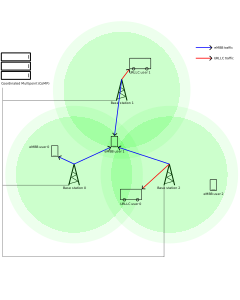
\includegraphics[width=0.5\textwidth]{model_multicell}
    \caption{Multicell model}
  \end{figure}
\end{frame}

\subsection{Spectrum Inefficiency}
\begin{frame}
  \frametitle{Spectrum Inefficiency}
  \begin{itemize}
    \item Dedicated URLLC bandwidth wastes spectral resources significantly in multicell systems.
      \begin{itemize}
        \item If $2$ subchannels of each base station are dedicated to URLLC traffic, then we would have $6$ subchannels sitting \highlight{idle for most of the time} in the aforementioned scenario.
      \end{itemize}
  \end{itemize}
\end{frame}

\begin{frame}
  \begin{itemize}
    \item This problem can be addressed by leveraging URLLC superposition/puncturing scheme. % TODO citations
    \item URLLC superposition scheme employs 5G NOMA SIC, whose performance equals to puncturing when the considered eMBB and URLLC users have the same channel gain. % TODO citations and example
    \item URLLC puncturing scheme is discussed here.
  \end{itemize}
\end{frame}

\begin{frame}
  \begin{figure}
    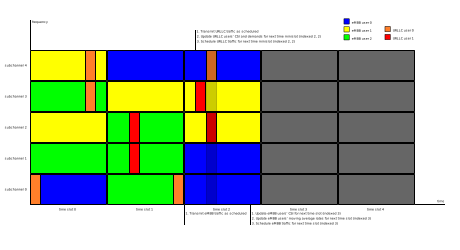
\includegraphics[width=1.05\textwidth]{framework_singlecell}
    \caption{Singlecell framework}
  \end{figure}
\end{frame}

\section{Problem}
\begin{frame}
  \frametitle{Problem}
  \tiny
  \begin{maxi!}
    {\embbRaVec, \embbLaVec, \urllcRaVec, \urllcLaVec}{\sum_{\embbUser}{\utilityCompositeFunction{\embbAverageRateRandOne}}\label{pb:problem0}}
    {}{}
    \addConstraint
      {\sum_{\baseStation}{\embbLaThree}}
      {\leq \multiconnectivityCapacity\label{pb:problem1}}
      {\forall\embbUser \forall\timeSlot}
    \addConstraint
      {\embbRaFour}
      {\leq \embbLaThree\label{pb:problem2}}
      {\forall\embbUser \forall\timeSlot \forall\baseStation \forall\subchannel}
    \addConstraint
      {\embbLaThree}
      {\in \setDst{0, 1}\label{pb:problem3}}
      {\forall\embbUser \forall\timeSlot \forall\baseStation}
    \addConstraint
      {\sum_{\embbUser}{\embbRaFour}}
      {\leq 1\label{pb:problem4}}
      {\forall\timeSlot \forall\baseStation \forall\subchannel}
    \addConstraint
      {\embbRaFour}
      {\in \setDst{0, 1}\label{pb:problem5}}
      {\forall\embbUser \forall\timeSlot \forall\baseStation \forall\subchannel}
    \addConstraint
      {\sum_{\baseStation}{\urllcLaFour}}
      {\leq 1\label{pb:problem6}}
      {\forall\urllcUser \forall\timeSlot \forall\timeMinislot}
    \addConstraint
      {\urllcRaSix}
      {\leq \urllcLaFour\label{pb:problem7}}
      {\forall\urllcUser \forall\embbUser \forall\timeSlot \forall\timeMinislot \forall\baseStation \forall\subchannel}
    \addConstraint
      {\urllcLaFour}
      {\in \setDst{0, 1}\label{pb:problem8}}
      {\forall\urllcUser \forall\timeSlot \forall\timeMinislot \forall\baseStation}
    \addConstraint
      {\sum_{\urllcUser}{\urllcRaSix}}
      {\leq \embbRaFour\label{pb:problem9}}
      {\forall\embbUser \forall\timeSlot \forall\timeMinislot \forall\baseStation \forall\subchannel}
    \addConstraint
      {\urllcRateRandThree}
      {\geq \demandRandThree\label{pb:problem10}}
      {\forall\urllcUser \forall\timeSlot \forall\timeMinislot}
    \addConstraint
      {\urllcRaSix}
      {\in \setDst{0, 1}\label{pb:problem11}}
      {\forall\urllcUser \forall\embbUser \forall\timeSlot \forall\timeMinislot \forall\baseStation \forall\subchannel}
  \end{maxi!}
\end{frame}

\begin{frame}
  \begin{itemize}
    \item The system maximizes eMBB traffic's total average rate and fairness \eqref{pb:problem0}.
    \item For each time slot, the system
      \begin{itemize}
        \item complies with the multiconnectivity capabilities of eMBB users \eqref{pb:problem1}.
        \item schedules a subchannel to an eMBB user only if it associates the corresponding base station to the user \eqref{pb:problem2}.
        \item either un-associates or associates a base station to an eMBB user \eqref{pb:problem3}.
        \item schedules a subchannel to at most one eMBB user \eqref{pb:problem4}.
        \item either un-schedules or schedules a subchannel to an eMBB user \eqref{pb:problem5}.
      \end{itemize}
  \end{itemize}
\end{frame}

\begin{frame}
  \begin{itemize}
    \item For each time minislot, the system
      \begin{itemize}
        \item associates at most one base station to a URLLC user \eqref{pb:problem6}.
        \item schedules a subchannel to a URLLC user only if it associates the corresponding base station to the user \eqref{pb:problem7}.
        \item either un-associates or associates a base station to a URLLC user \eqref{pb:problem8}.
        \item schedules a subchannel to at most one URLLC user, and punctures the subchannel for a URLLC user only if it schedules the subchannel to the corresponding eMBB user \eqref{pb:problem9}\proofFootnote.
        \item serves demands of URLLC users without delays \eqref{pb:problem10}.
        \item employs URLLC puncturing scheme instead of superposition \eqref{pb:problem11}.
      \end{itemize}
  \end{itemize}
\end{frame}

\begin{frame}
  \begin{itemize}
    \item Do note that current eMBB users' rate models for URLLC puncturing scheme in the literature are mostly non-linear \cite{BMATAMHH21}.
    \item Whilst proposed linear models are either intractable \cite{YZR21} or inappropriate \cite{AVS20} for discrete subchannel scheduling with multiple URLLC users.
  \end{itemize}
\end{frame}

\begin{frame}
  \frametitle{eMBB Problem}
  \begin{maxi!}
    {\embbRaVec, \embbLaVec}{\sum_{\embbUser}{\utilityCompositeFunction{\embbAverageRateRandOne}}}
    {}{}
    \addConstraint
      {\sum_{\baseStation}{\embbLaThree}}
      {\leq \multiconnectivityCapacity}
      {\forall\embbUser \forall\timeSlot}
    \addConstraint
      {\embbRaFour}
      {\leq \embbLaThree}
      {\forall\embbUser \forall\timeSlot \forall\baseStation \forall\subchannel}
    \addConstraint
      {\embbLaThree}
      {\in \setDst{0, 1}}
      {\forall\embbUser \forall\timeSlot \forall\baseStation}
    \addConstraint
      {\sum_{\embbUser}{\embbRaFour}}
      {\leq 1}
      {\forall\timeSlot \forall\baseStation \forall\subchannel}
    \addConstraint
      {\embbRaFour}
      {\in \setDst{0, 1}}
      {\forall\embbUser \forall\timeSlot \forall\baseStation \forall\subchannel}
  \end{maxi!}
\end{frame}

\begin{frame}
  \frametitle{Relaxed eMBB Problem}
  \begin{maxi!}
    {\embbRaVecRelax, \embbLaVecRelax}{\sum_{\embbUser}{\utilityCompositeFunction{\embbAverageRateRandOneRelax}}}
    {}{}
    \addConstraint
      {\sum_{\baseStation}{\embbLaThreeRelax}}
      {\leq \multiconnectivityCapacity}
      {\forall\embbUser \forall\timeSlot}
    \addConstraint
      {\embbRaFourRelax}
      {\leq \embbLaThreeRelax}
      {\forall\embbUser \forall\timeSlot \forall\baseStation \forall\subchannel}
    \addConstraint
      {\embbLaThreeRelax}
      {\leq 1}
      {\forall\embbUser \forall\timeSlot \forall\baseStation}
    \addConstraint
      {\embbLaThreeRelax}
      {\geq 0}
      {\forall\embbUser \forall\timeSlot \forall\baseStation}
    \addConstraint
      {\sum_{\embbUser}{\embbRaFourRelax}}
      {\leq 1}
      {\forall\timeSlot \forall\baseStation \forall\subchannel}
    \addConstraint
      {\embbRaFourRelax}
      {\geq 0}
      {\forall\embbUser \forall\timeSlot \forall\baseStation \forall\subchannel}
  \end{maxi!}
\end{frame}

\begin{frame}
  \frametitle{Gradient Problem}
  \begin{maxi!}
    {\embbRaVecOneRelaxCur, \embbLaVecOneRelaxCur}{\sum_{\embbUser}{\frac{\embbRateTwoRelaxCur}{\embbMovingAverageRateTwoRelaxCur}}}
    {}{}
    \addConstraint
      {\sum_{\baseStation}{\embbLaThreeRelaxCur}}
      {\leq \multiconnectivityCapacity}
      {\forall\embbUser}
    \addConstraint
      {\embbRaFourRelaxCur}
      {\leq \embbLaThreeRelaxCur}
      {\forall\embbUser \forall\baseStation \forall\subchannel}
    \addConstraint
      {\embbLaThreeRelaxCur}
      {\leq 1}
      {\forall\embbUser \forall\baseStation}
    \addConstraint
      {\embbLaThreeRelaxCur}
      {\geq 0}
      {\forall\embbUser \forall\baseStation}
    \addConstraint
      {\sum_{\embbUser}{\embbRaFourRelaxCur}}
      {\leq 1}
      {\forall\baseStation \forall\subchannel}
    \addConstraint
      {\embbRaFourRelaxCur}
      {\geq 0}
      {\forall\embbUser \forall\baseStation \forall\subchannel}
  \end{maxi!}
\end{frame}

\begin{frame}
  \begin{itemize}
    \item The relaxed moving average rate of eMBB user is defined based on exponential moving average (EMA) as
      \begin{equation}
        \embbMovingAverageRateTwoRelax =
          \begin{cases}
            \frac{1}{\timeSlotsNum} \sum_{\baseStation, \subchannel}{\frac{1}{\embbUsersNum} \embbPeakRateFour} &\timeSlot = 0\\
            \left(1 - \smoothingFactor\right) \embbMovingAverageRateTwoRelaxDecrement + \smoothingFactor \embbRateTwoRelaxDecrement &\nonzeroTimeSlots
          \end{cases} \bpsl \forall\embbUser.
      \end{equation}
  \end{itemize}
\end{frame}

\begin{frame}
  \begin{itemize}
    \item The initial value of which is defined by the feasible policy $\tuple{\embbRaVecRelaxCandidate, \embbLaVecRelaxCandidate}$ for the relaxed eMBB problem where\proofFootnote
      \begin{align}
        \embbRaFourRelaxCandidate &=
          \begin{cases}
            \frac{1}{\embbUsersNum} &\timeSlot = 0\\
            0 &\nonzeroTimeSlots
          \end{cases} &\forall\embbUser \forall\baseStation \forall\subchannel,\\
        \embbLaThreeRelaxCandidate &=
          \begin{cases}
            \frac{\multiconnectivityCapacity}{\baseStationsNum} &\timeSlot = 0\\
            0 &\nonzeroTimeSlots
          \end{cases} &\forall\embbUser \forall\baseStation.
      \end{align}
  \end{itemize}
\end{frame}

\begin{frame}
  \begin{itemize}
    \item Our set of policy(ies) is defined as
      \begin{equation}
        \policySet = \left\{\tuple{\embbRaVecCandidate, \embbLaVecCandidate} \subjectTo
          \begin{aligned}
            \forall\timeSlot \colon \tuple{\embbRaVecOneCandidate, \embbLaVecOneCandidate} \text{ is a basic optimal point}\\
            \text{of $\timeSlot^{th}$ gradient problem}
          \end{aligned} \right\}.
      \end{equation}
  \end{itemize}
\end{frame}

\begin{frame}
  \begin{itemize}
    \item $\tuple{\embbRaVecCandidate, \embbLaVecCandidate}$ is an asymptotically optimal policy for the eMBB problem\proofFootnote.
  \end{itemize}
\end{frame}


\begin{frame}
  \frametitle{References}
  \printbibliography[heading=none]
\end{frame}

\end{document}
